\documentclass{article}
\usepackage{graphicx}
\usepackage{tcolorbox}
\usepackage[utf8]{inputenc}
\usepackage[spanish]{babel}
\usepackage{hyperref}
\usepackage{graphicx}
\usepackage{epstopdf} %%package to overcome problem with eps in pdf files



\newcommand{\instruction}[1]{\textsc{\begin{tcolorbox}#1\end{tcolorbox}}}

\begin{document}

\title{World Development Indicators}
\author{Francisco Clavero, Vicente Oyanedel, Fabián Souto}

\maketitle

\section{Goal}
La meta de este proyecto es obtener los indicadores más presentes en los países y años; esto último (presencia en años) es que se tenga consistencia en el tiempo de cada indicador por país. Con los indicadores seleccionados se desea generar visualizaciones de nuestro país, Chile, y países escogidos para su comparación de distintas partes del mundo; tales como EEUU, China, Portugal y Perú. El primero y el segundo por ser potencias mundiales pero de continentes distintos, Portugal para comparar con un país similar a Chile pero Europeo y Perú para comparar con un país vecino.\\

A partir de los resultados se hará un análisis de éstos y poder ver correlaciones entre hechos históricos, y los países entre sí.\\

\section{Data}
El dataset escogido corresponde a la base da datos \href{https://www.kaggle.com/worldbank/world-development-indicators}{World Development Indicators} de \textit{Kaggle}. Esta contiene los valores de distintos indicadores económicos de más de 243 países del mundo, tales como su PIB, distintas mediciones demográficas y de emiciones de CO2. La base de datos está disponible tanto en formato \textit{sqlite} como en una serie de archivos CSV. Para poder manejarlos en el sistema distribuido se trabajó con el archivo \textit{Indicators.csv}, que contiene los valores de los indicadores y tiene un tamaño de 560 MB. \\

\section{Methods}
En primer lugar, se implementa una serie de programas en \textbf{Pig} para la extracción y analisis de los datos. \\
Luego, se implementa un script en \textbf{Python} para generar las visualizaciones de los datos generados en Pig.\\

\paragraph{Pig:}
Se implementaron los siguientes archivos, que pueden ser encontrados en el \href{https://github.com/programasut/world-dev-analysis/tree/master/pig}{repositorio de código}:
\begin{enumerate}
	\item year\_count.pig: Para obtener la cantidad de años que hay en los datos. Esto se utilizó en un comienzo para encontrar los paises que tuvieran todos los indicadores. 
	\item country\_count.pig: Para obtener la cantidad de países que hay en los datos. Se utilizó, como el anterior, en la busqueda de paises con todos los indicadores.
	\item nice\_indicators.pig: Para obtener una lista de indicadores para los paises, tal que tuvieran una muestra suficientemente grande. Éste resultado se logró sumando las cuentas de los programas anteriores para así obtener una noción de la cantidad de indicadores por pais por año, y luego se fija un numero levemente menor a éste.
	\item general\_script.pig: Filtrar los datos fuente (Kaggle) por los países que se eligieron para hacer el analisis.
\end{enumerate}
Se llega a esta solución despues de intentar obtener los países que tuvieran todos los indicadores que Chile, dentro de un periodo de tiempo. Solución que se descarta después de intentar de manera ardua programar un nested foreach de divsersas maneras, para finalmente descubrir que el lenguaje no lo permitía.\\

Otra dificultad ocurre al cargar los datos en formato csv, el cual posee el carácter separador en el texto. Para lo cual descargó la extensión Piggybank.pig, la cual posee un parser de CSV que funciona perfectamente.\\
\paragraph{Python:}
Obtenidos la lista de indicadores suficientes y los datos filtrados por los países; se prosiguió a importar los datos en Python y hacer visualizaciones (con pyplot) para cada indicador en función del tiempo. Esto se hace en el script que se encuentra en el \href{https://github.com/programasut/world-dev-analysis/tree/master/python}{repositorio de código.}
\section{Results}
Al comenzar a explorar y analisar los datos mediante Pig, se observa:
\begin{enumerate}
	\item No hay ningún país con todos los indicadores.
	\item Con más de 13000 habían muy pocos.
	\item Los indicadores que más tenían países eran muy pocos, y algunos no tan relevantes.
\end{enumerate}
En base a ésto se eligió los atributos más relevantes para nosotros. Luego se graficaron mediante Python en las visualizaciones que se presentan en el anexo.\\

Del análisis que vá más allá de lo que se deja a ver a simple vista, se concluye:\\
\\
\paragraph{Población total vs Tiempo:}
Figura \ref{fig:12}\\
Se nota que China crece más rapido y gana en tamaño al resto.\\

Al hacer Zoom (figura \ref{fig:13})se puede dilusidar la baja tasa de fertilidad en paises europes. Por otro lado, Perú tiene tasa de fertilidad grande. \\
Se puede apoyar en el siguiente grafico: figura \ref{fig:4}.

\paragraph{Producto interno bruto vs Tiempo:}
Figura \ref{fig:6}.\\
Estados Unidos el mayor. Se observa un gran incremento de china.
La diferencia entre economías grandes y pequeñas se deja ver claramente.\\

Además, se pueden ver los efectos de las crisis economicas ocurridas en el periodo.\\

Al hacer Zoom (figura \ref{fig:7}), se deja ver que Chile se acerca a Portugal. Por otro lado, desde mediados de los 80' Chile gana repunte en su economía.

\paragraph{Población urbana vs Tiempo:}
Figura \ref{fig:1}.\\
De éste indicador se obtuvo un margen muy pequeño, que al graficarlo deja ver resultados bastante variantes; especialmente los Chinos que perdieron mucho entre el 65.\\
En contraste, portugal y china persiven un inmenso crecimiento entre el 73 y el 75.\\


\paragraph{Esperanza de vida vs Tiempo:}
Figura \ref{fig:2}.\\
Sórpresivamente, Chile muestra la mayor espectativa de vida.\\
China presiente un boom en los 70s.\\
Por su lado, Peru y chile son iguales muy similares. Teniendo Chile un crecimiento muy uniforme.\\


\paragraph{Hospital:}
Figura \ref{fig:5}.\\
Una conclusión interesante es que a medida que crece la poblacion, la cantidad de camas no aumenta de la misma manera y se ve disminuido.\\
Todos excepto estados unidos crecen más que este, dado que siempre dismnuye.

\paragraph{Exports:}
Figura \ref{fig:8}.\\
Se ven claramente las crisis. En los 80 china no hacía nada; montó las factorias y se disparó su crecimiento.\\
Se noto más la crisis de los 80 en comparacion al otro grafico. \\

Nuestra teoría es que China logró suplir las pérdidas mediante el consumo interno, por ello no se ve una baja en el producto interno bruto durante el mismo período.

\paragraph{Renovable:}
Figura \ref{fig:9}.\\
Malas noticias para el ambiente dado que se ve una clara tendencia a la baja. En especial Estados Unidos y China que demuestran muy bajo consumo de energía limpia. Aunque China muestra un leve crecimiento ultimamente; esperamos que siga así.

\section{Conclusion}

La generación de las visualizaciones fue bastante sencilla una vez que se tenían los datos a procesar. El manejo en python jugó de nuestro lado.\\
En un comienzo fue difícil realizar las consultas en \textit{PIG}, puesto que eran bastante estrictas y complejas. Luego notamos que para obtener los resultados deseados se podían generar de forma distintas -relajando las restricciones a los indicadores- y logramos sobrellevar nuestras dificultados con \textit{PIG}.\\
Para mejorar se podrían haber manejado los datos con \textit{MapReduce}, que da más libertades y así crear consultas más complejas.

\newpage
\section*{Appendix}



\begin{figure}[!h]
	\centering
	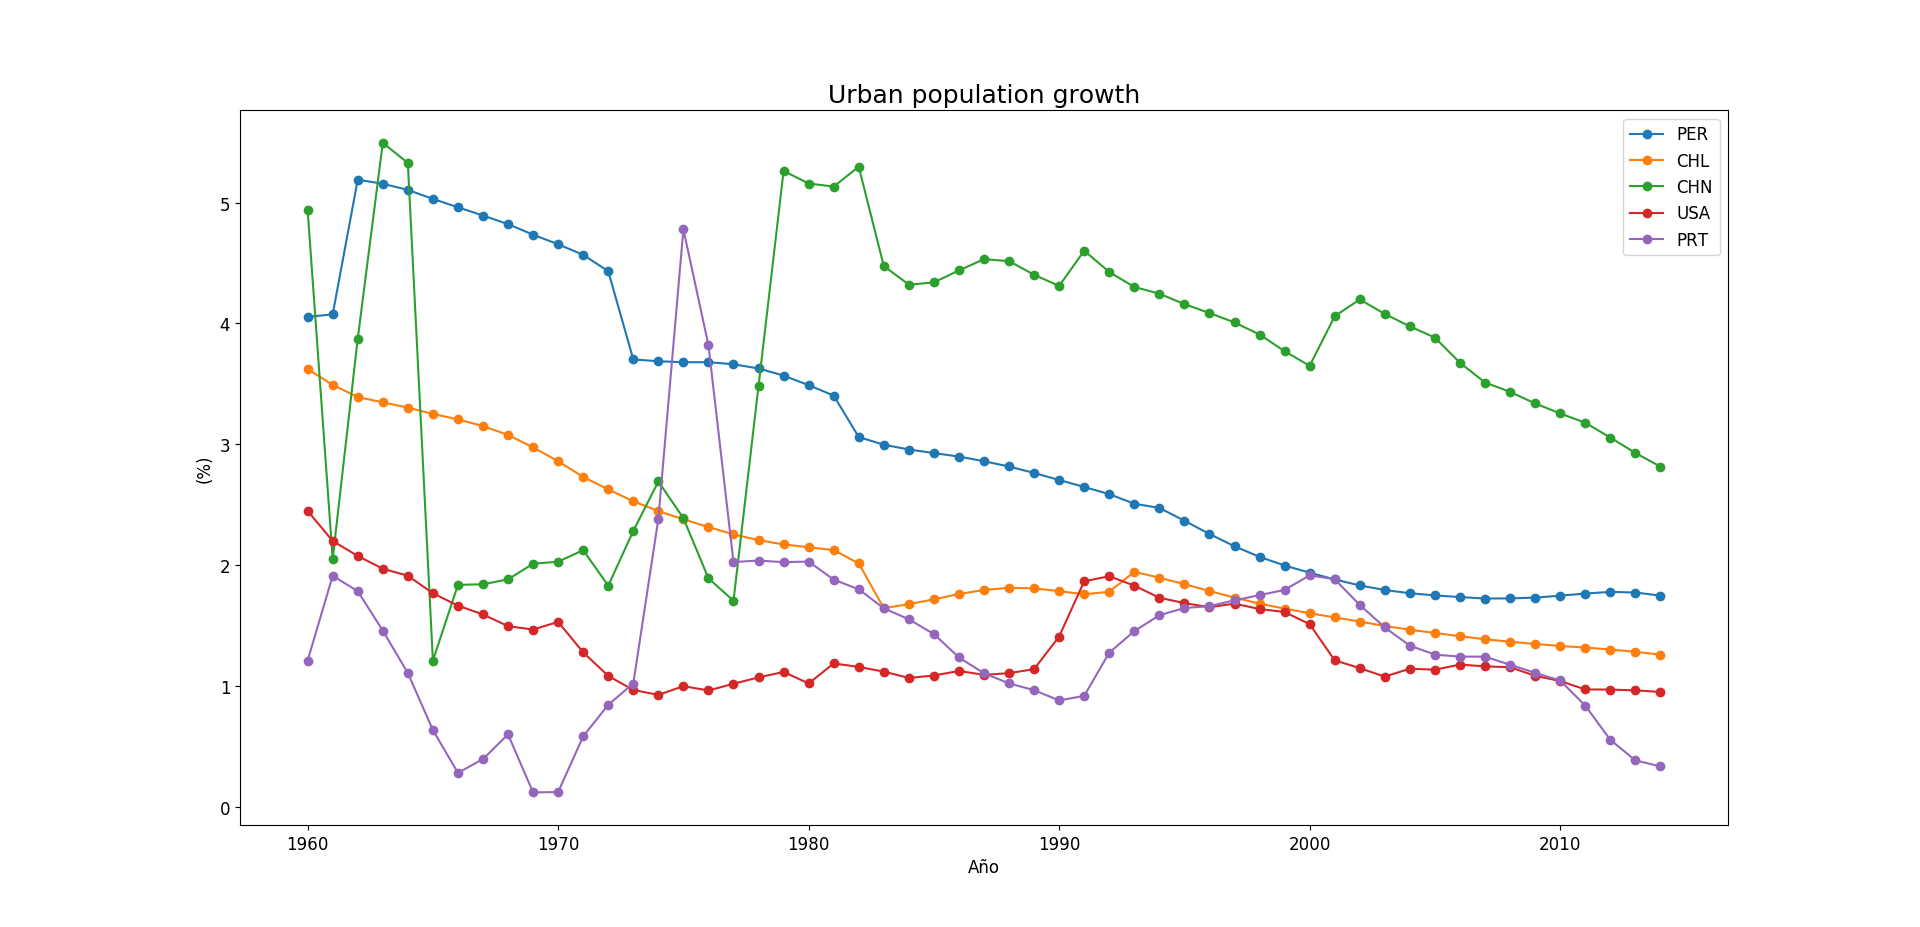
\includegraphics[scale=0.38]{images/2.png}
	\caption{Crecimiento de población urbana.}
	\label{fig:1}
\end{figure}

\begin{figure}
	\centering
	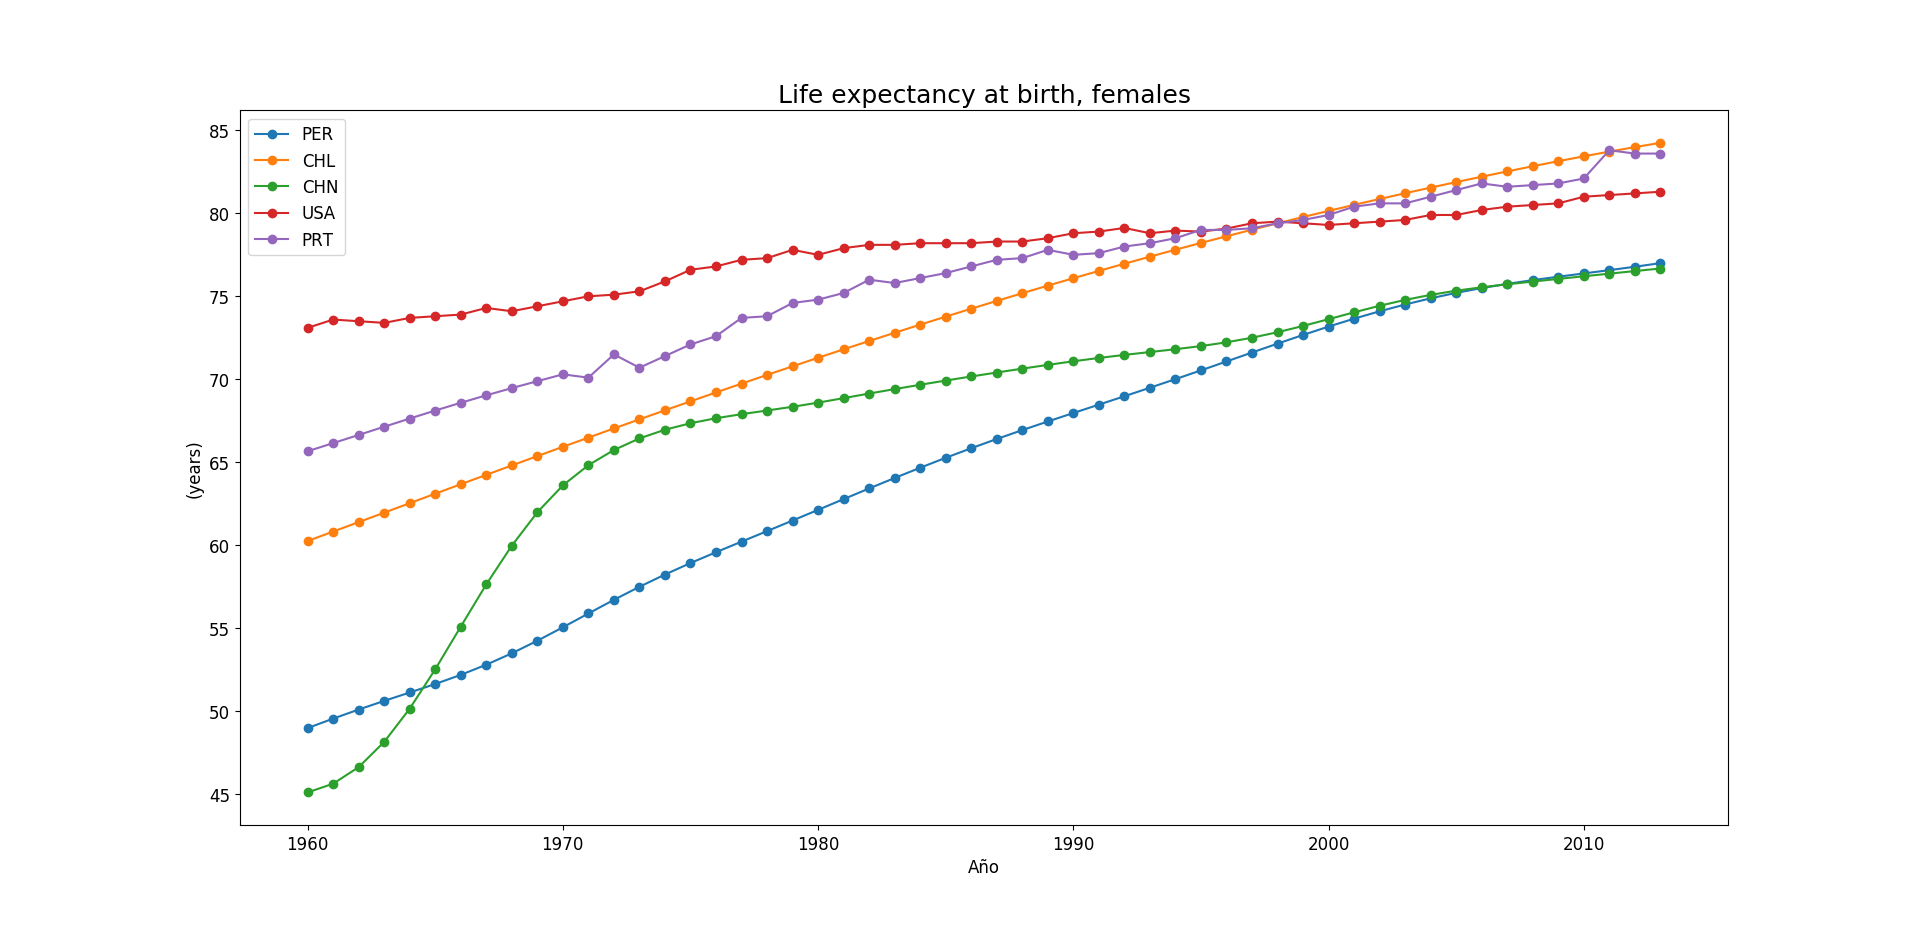
\includegraphics[scale=0.38]{images/figure_1.png}
	\caption{Esperanza de vida al nacer, mujeres.}
	\label{fig:2}
\end{figure}

\begin{figure}
	\centering
	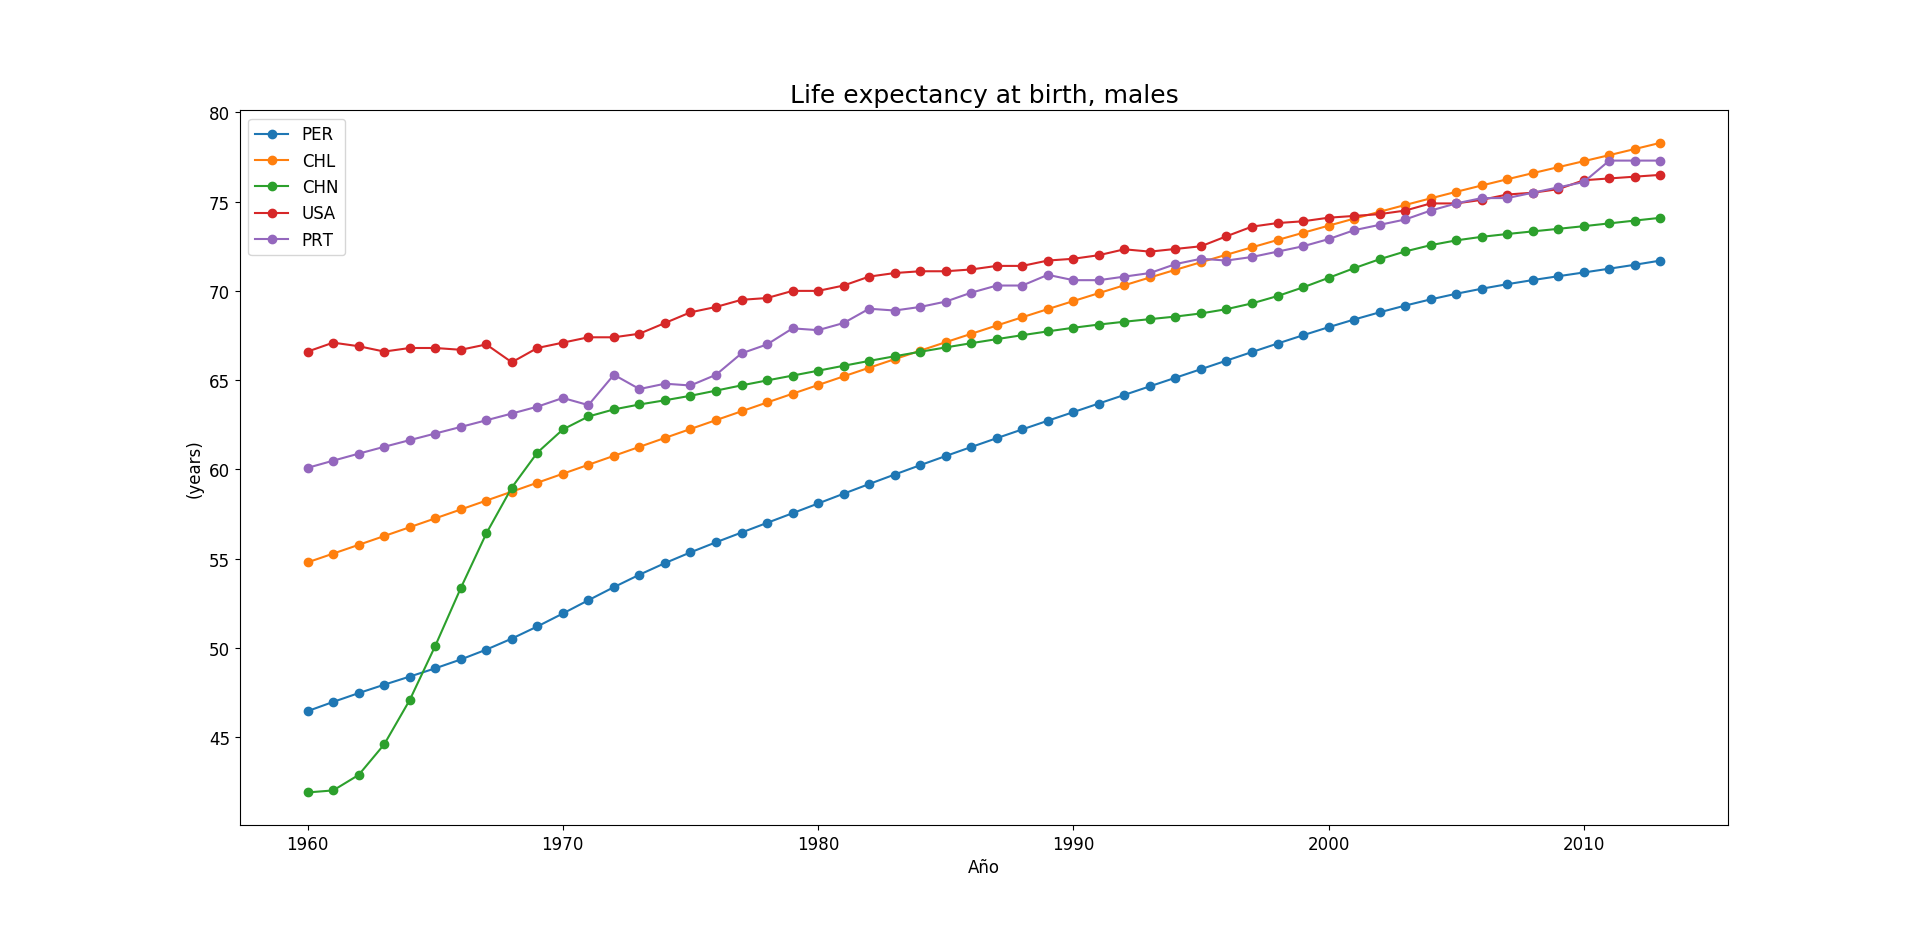
\includegraphics[scale=0.38]{images/figure_1-1.png}
	\caption{Esperanza de vida al nacer, hombres.}
	\label{fig:3}
\end{figure}

\begin{figure}
	\centering
	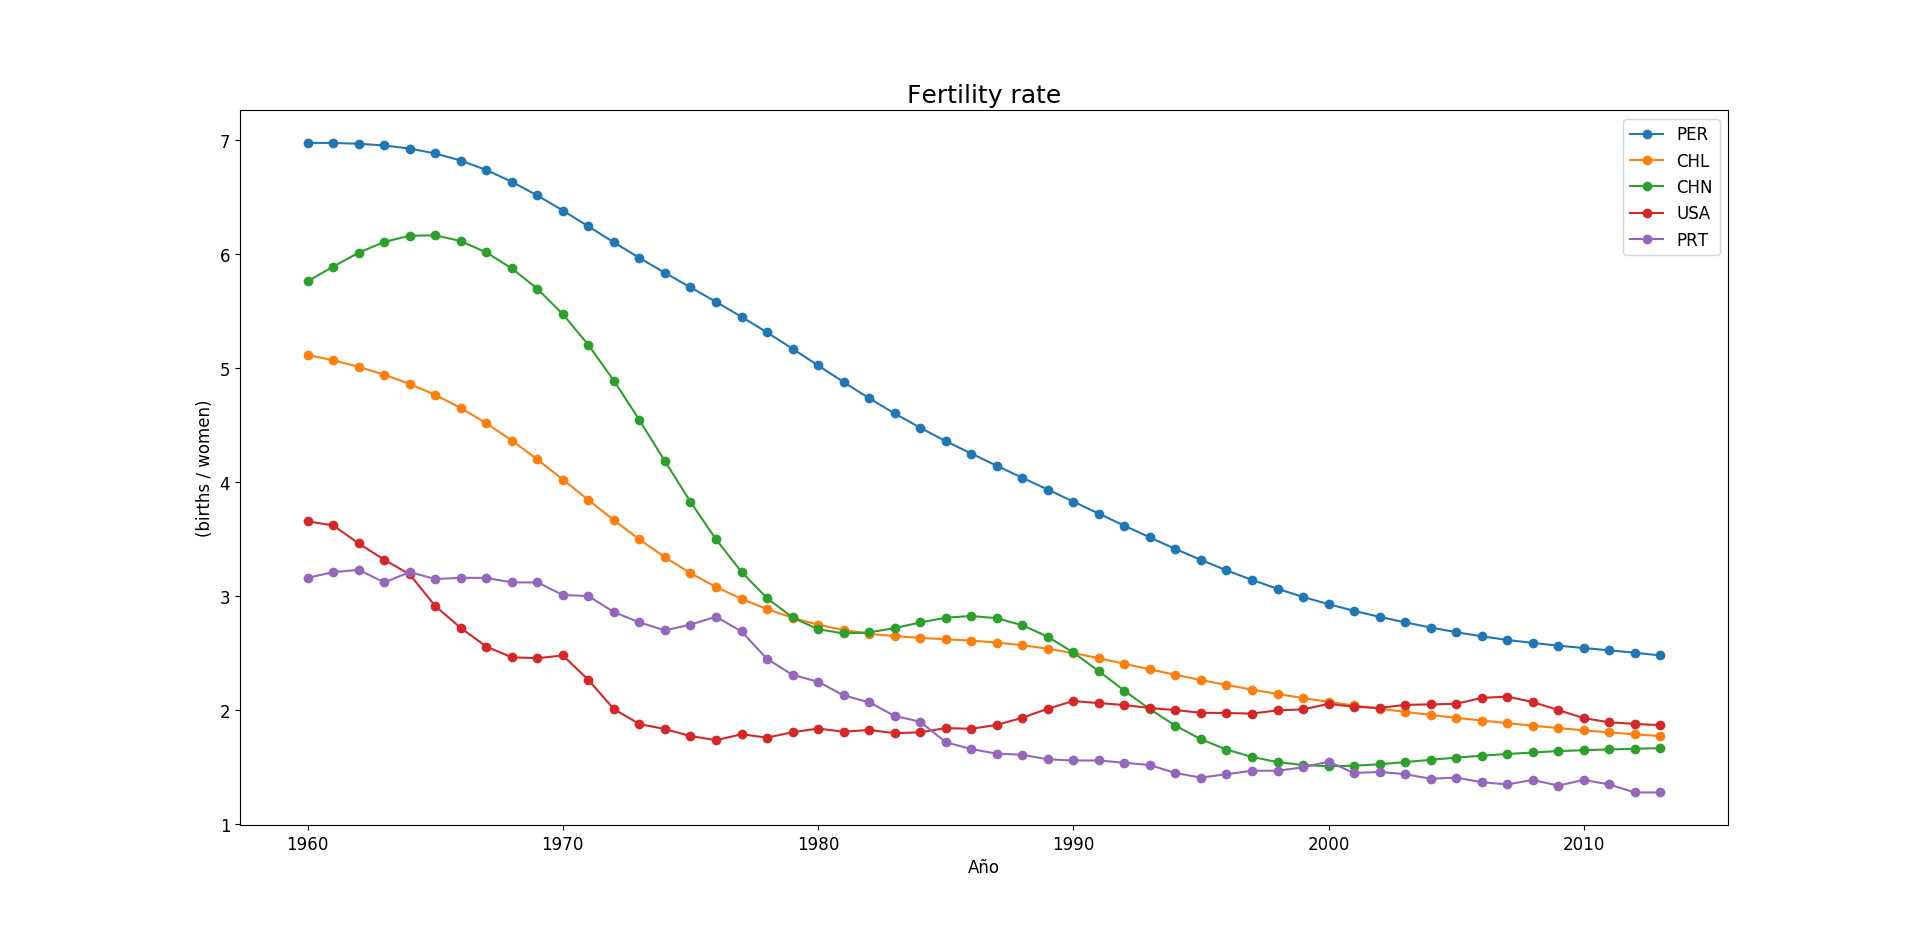
\includegraphics[scale=0.38]{images/figure_1-2.png}
	\caption{Fertilidad}
	\label{fig:4}
\end{figure}

\begin{figure}
	\centering
	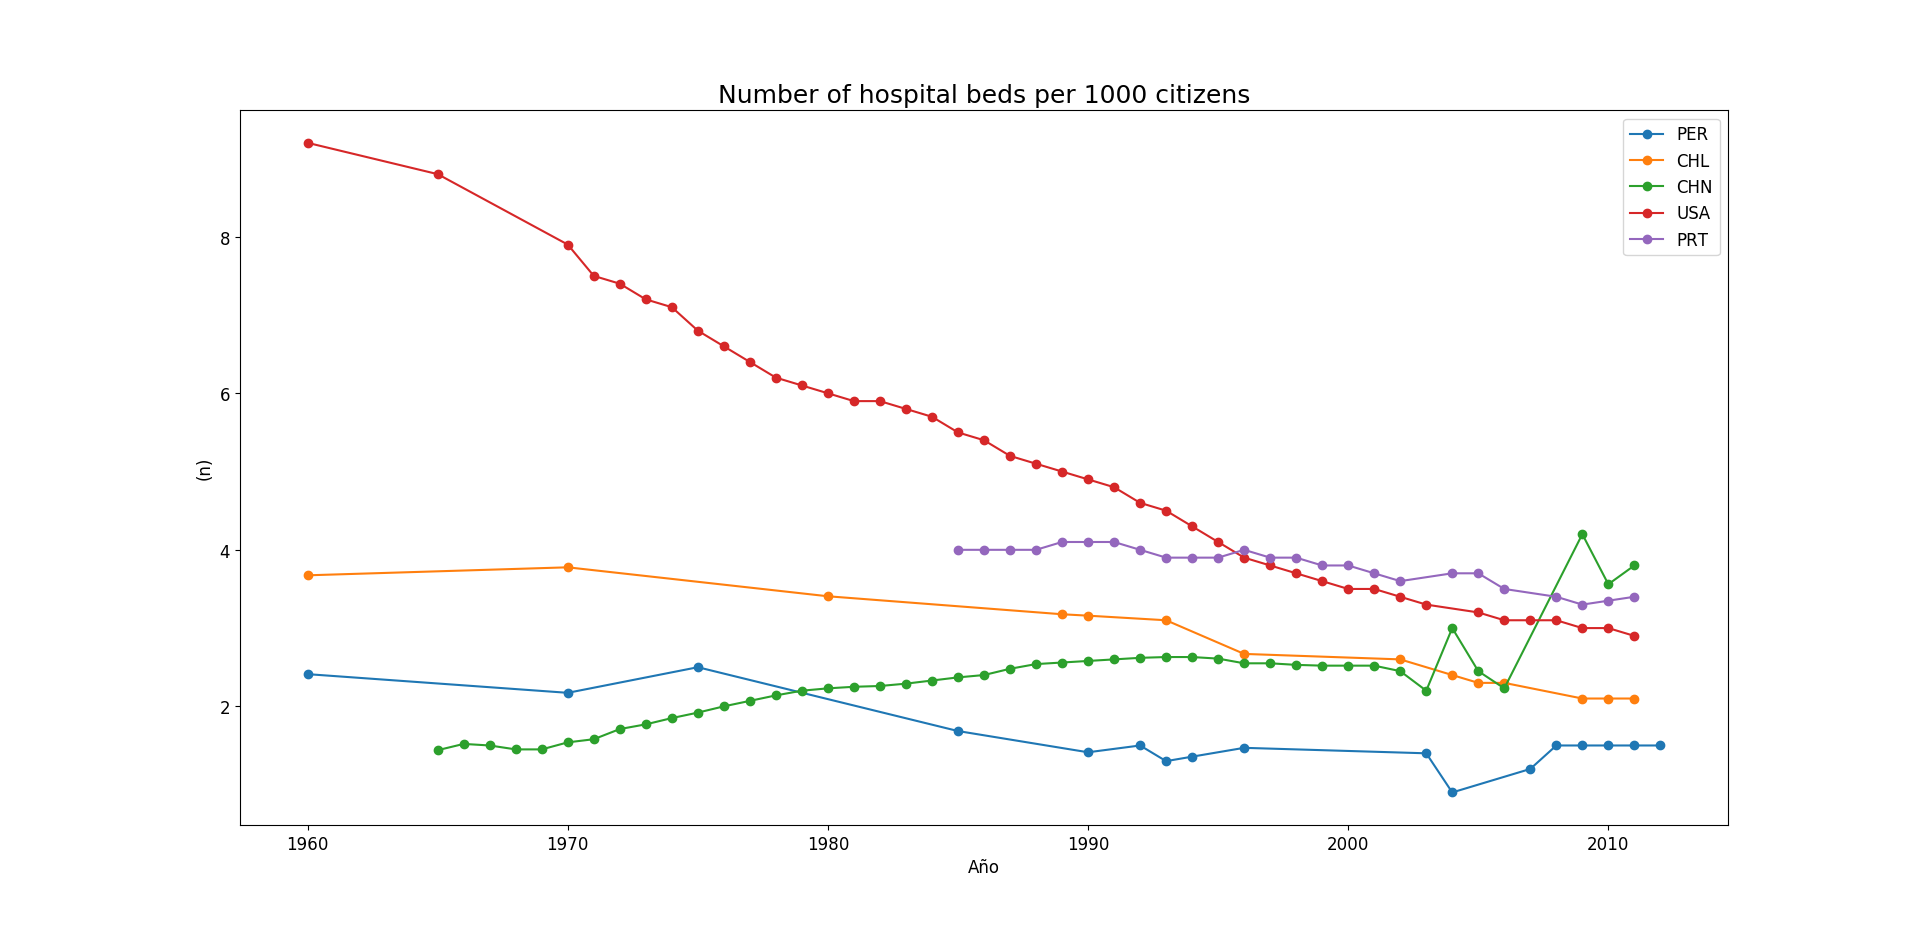
\includegraphics[scale=0.38]{images/figure_1-3.png}
	\caption{Numero de camas en hospitales por cada 1000 habitantes.}
	\label{fig:5}
\end{figure}

\begin{figure}
	\centering
	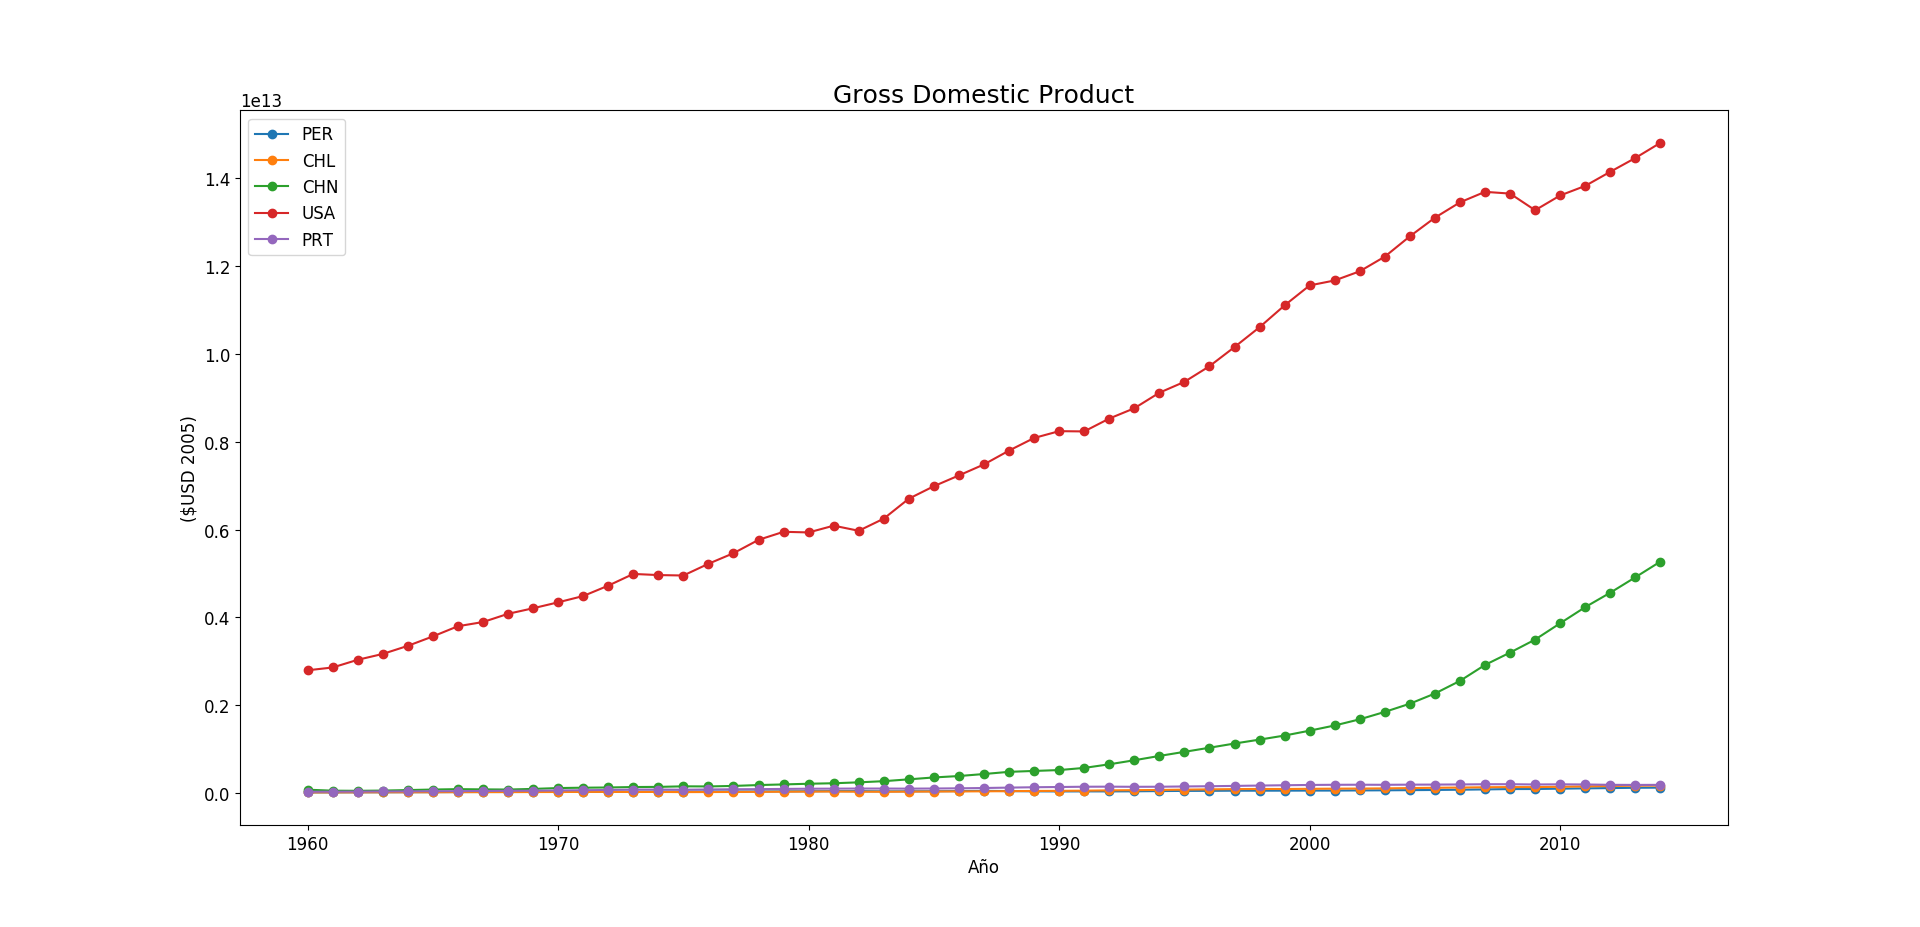
\includegraphics[scale=0.38]{images/figure_1-4.png}
	\caption{Producto interno bruto.}
	\label{fig:6}
\end{figure}

\begin{figure}
	\centering
	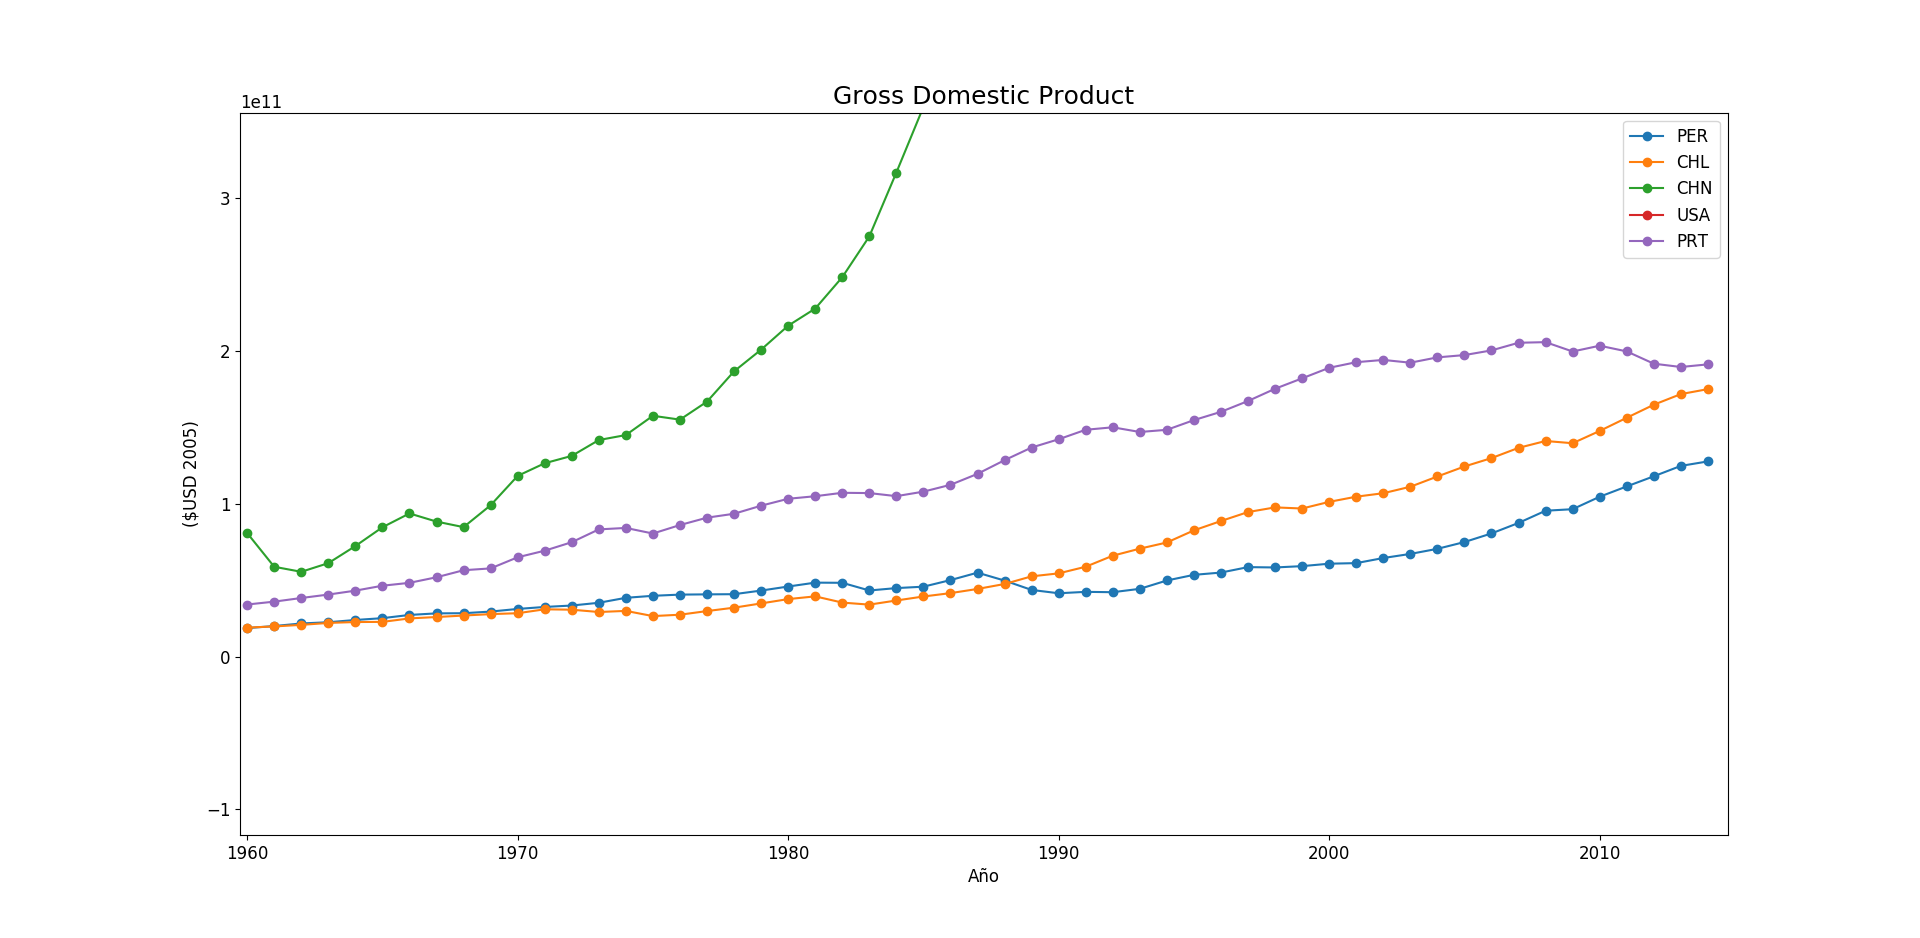
\includegraphics[scale=0.38]{images/a.png}
	\caption{Producto interno bruto: Zoom.}
	\label{fig:7}
\end{figure}


\begin{figure}
	\centering
	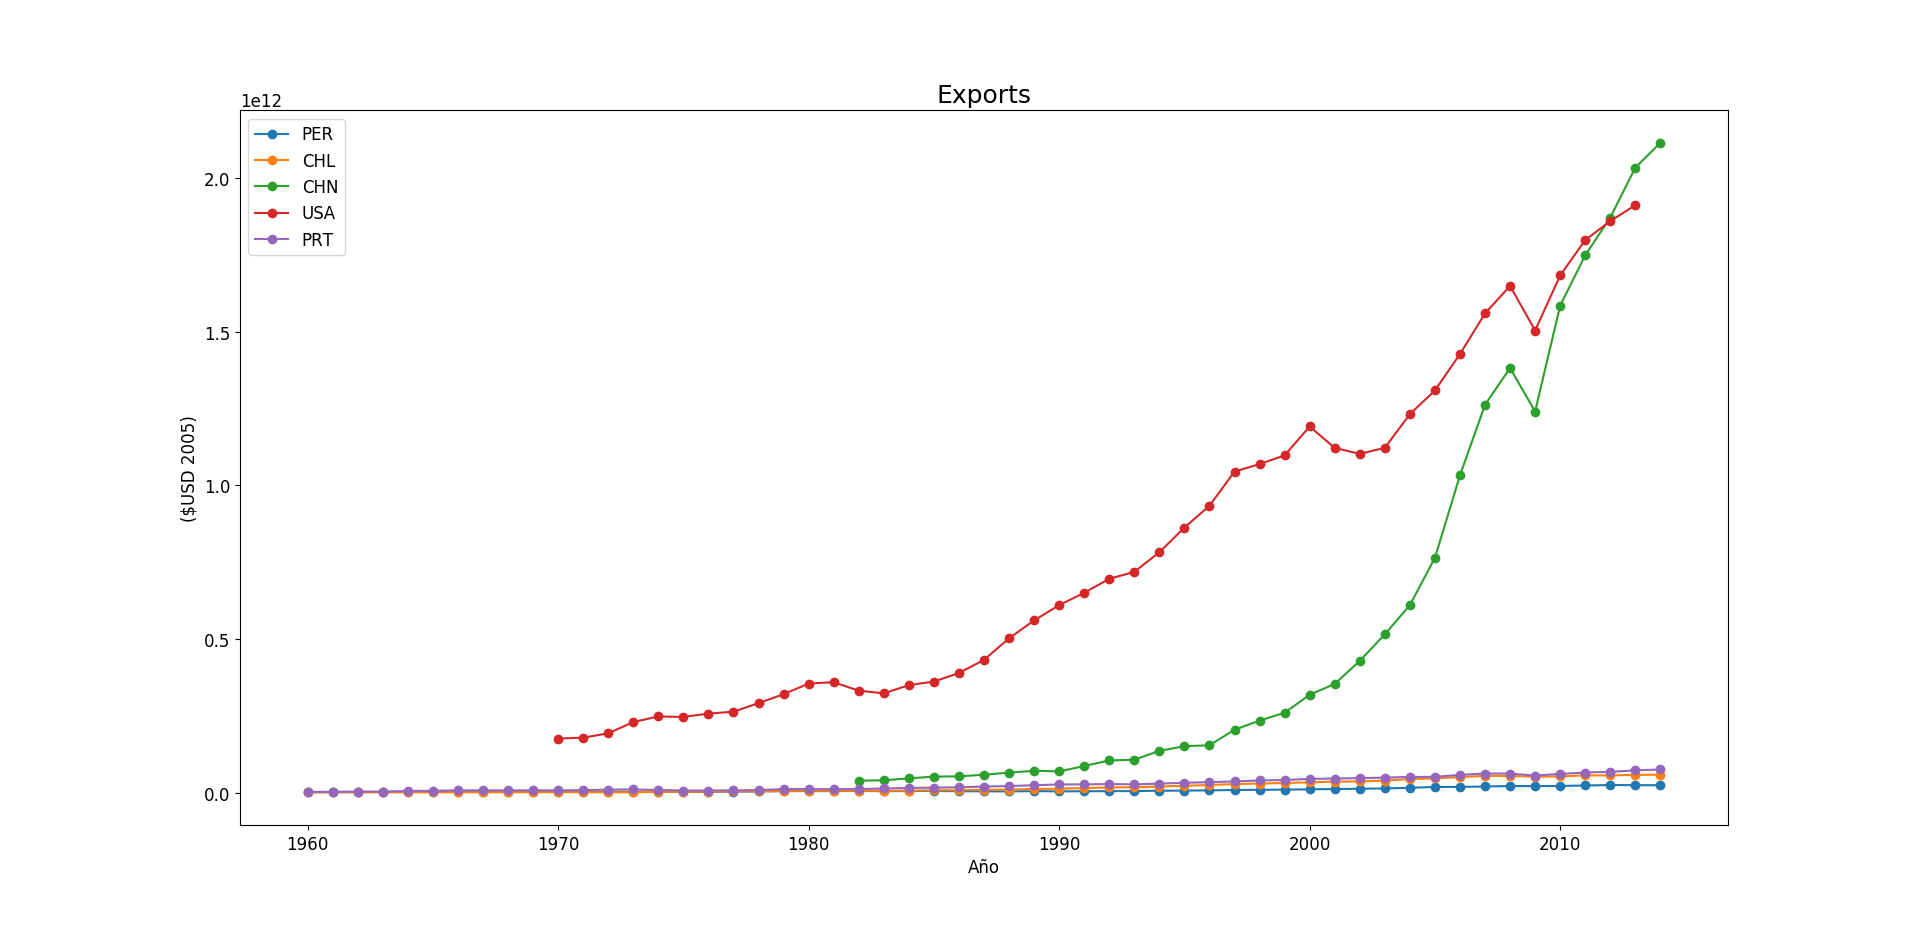
\includegraphics[scale=0.38]{images/figure_1-5.png}
	\caption{Exportaciones.}
	\label{fig:8}
\end{figure}

\begin{figure}
	\centering
	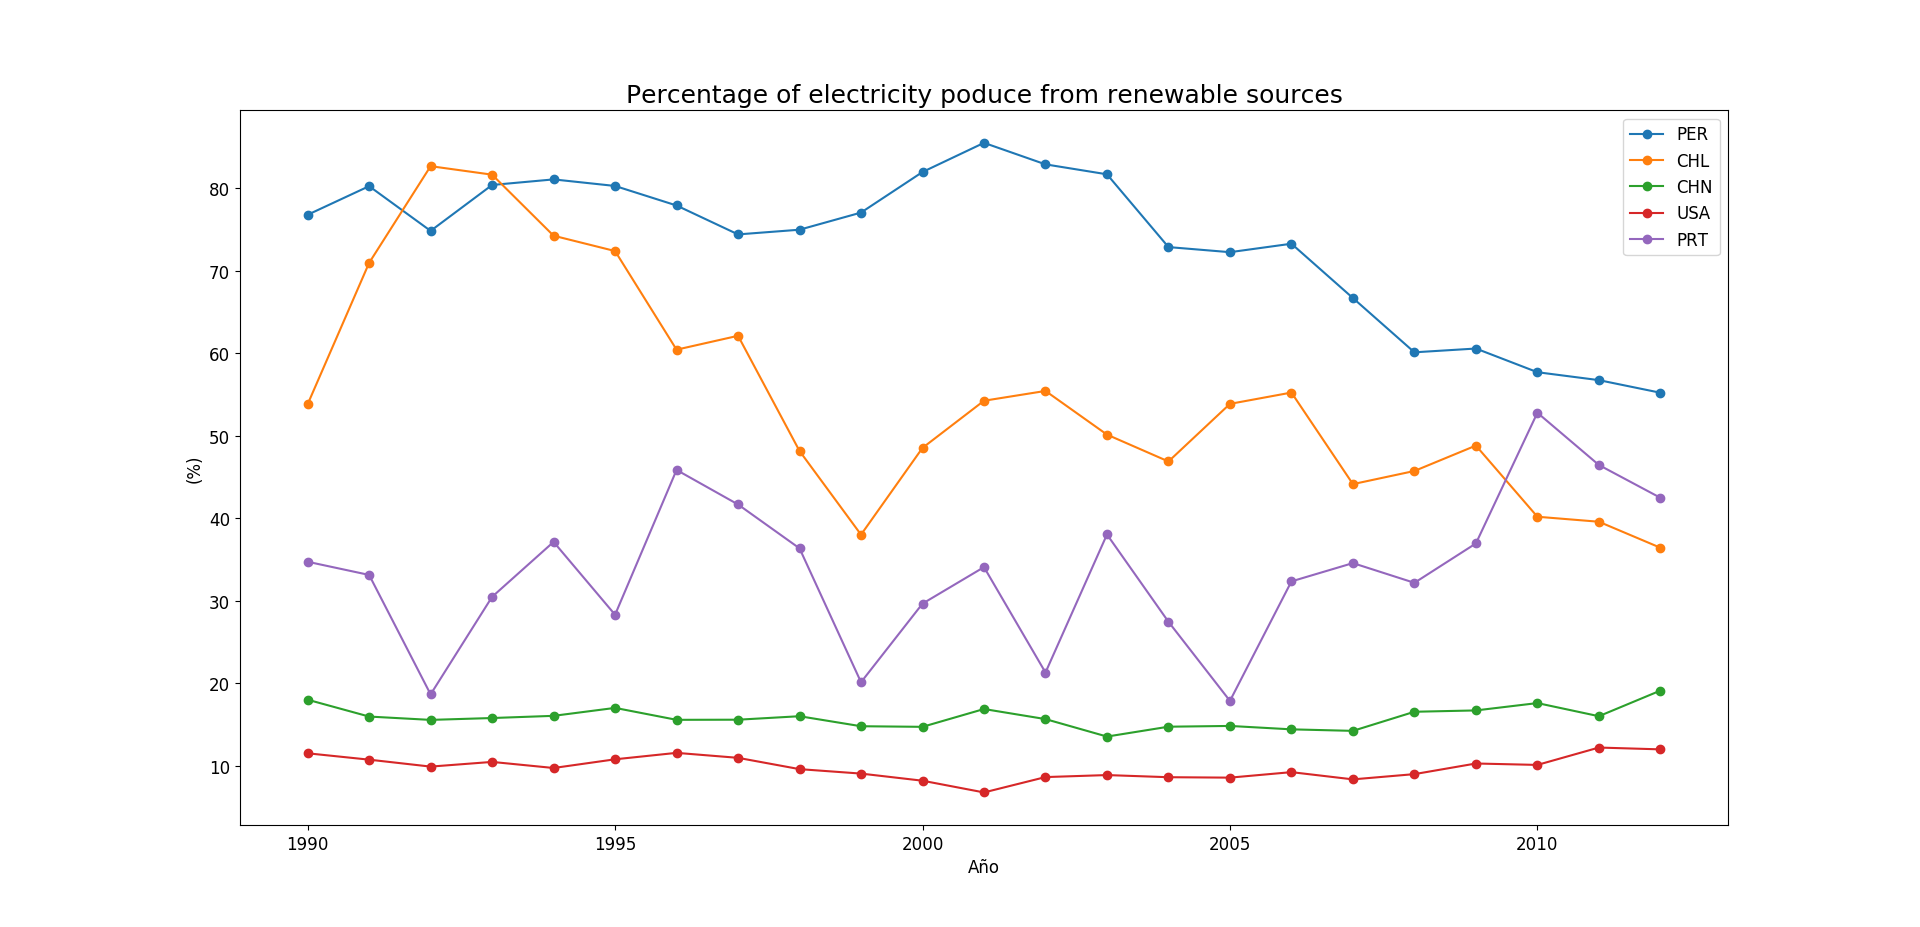
\includegraphics[scale=0.38]{images/figure_1-7.png}
	\caption{Porcentaje de electricidad producida por fuentes renovables.}
	\label{fig:9}
\end{figure}

\begin{figure}
	\centering
	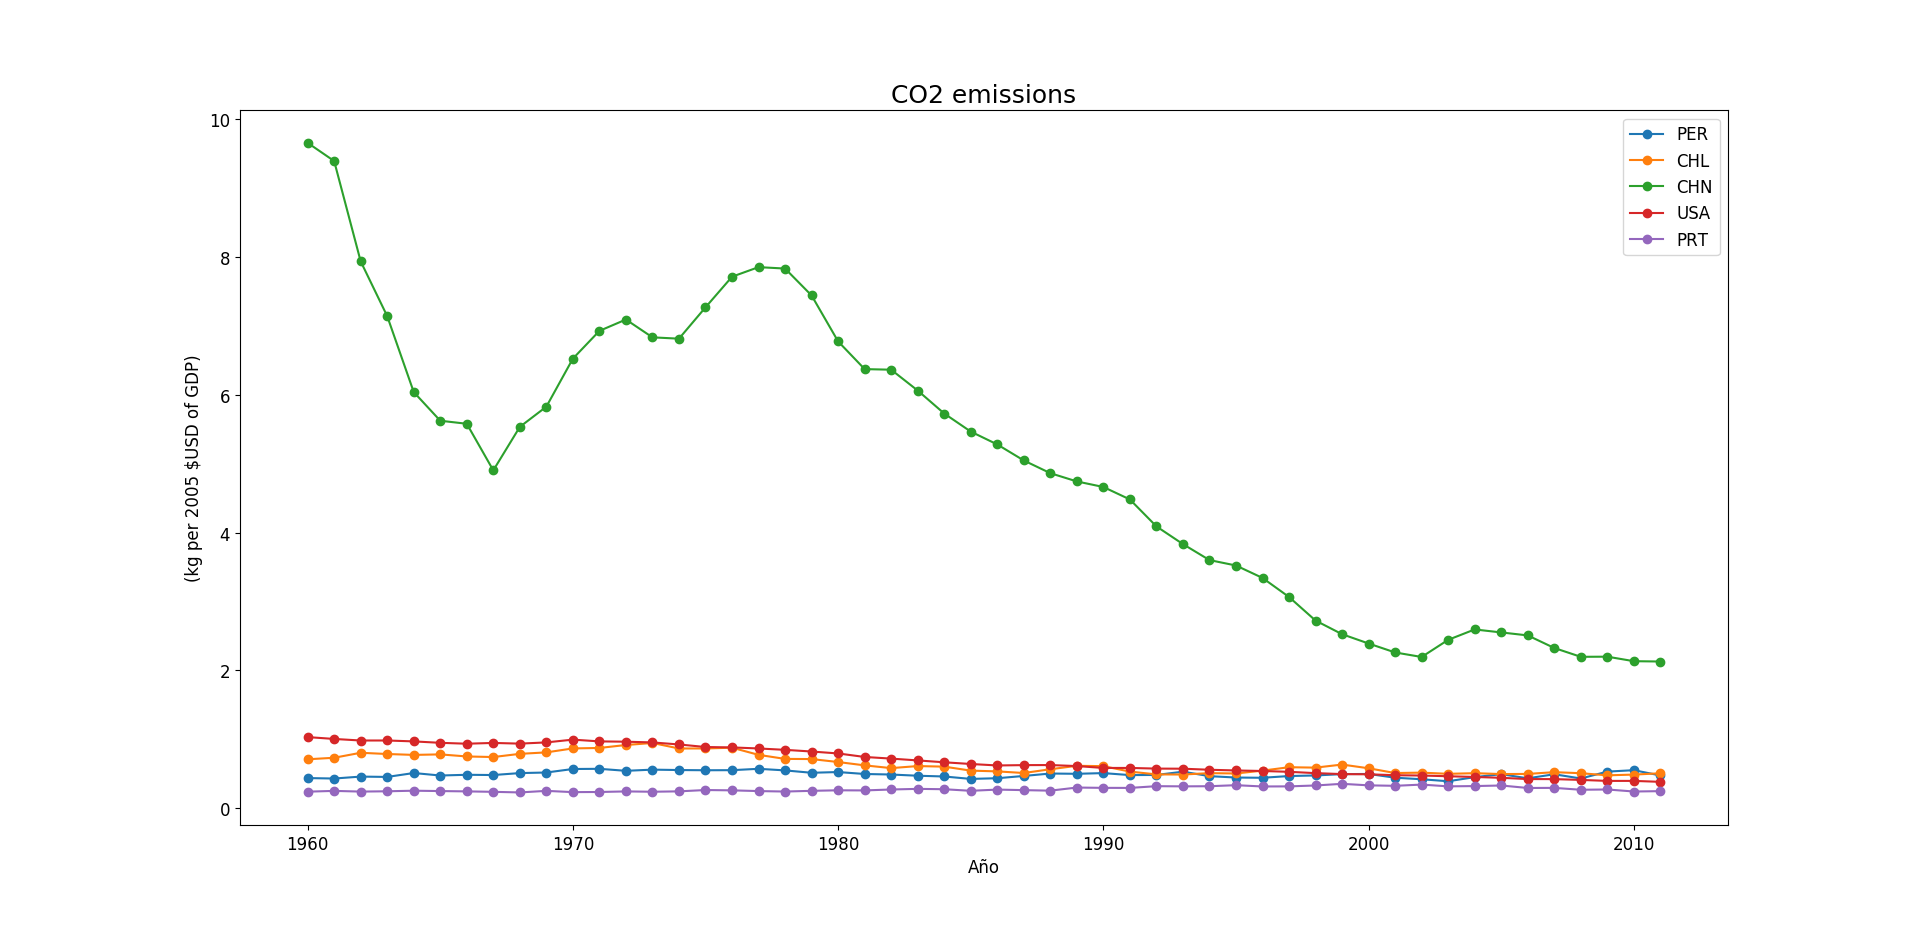
\includegraphics[scale=0.38]{images/figure_1-8.png}
	\caption{Emisiones de CO2.}
	\label{fig:10}
\end{figure}

\begin{figure}
	\centering
	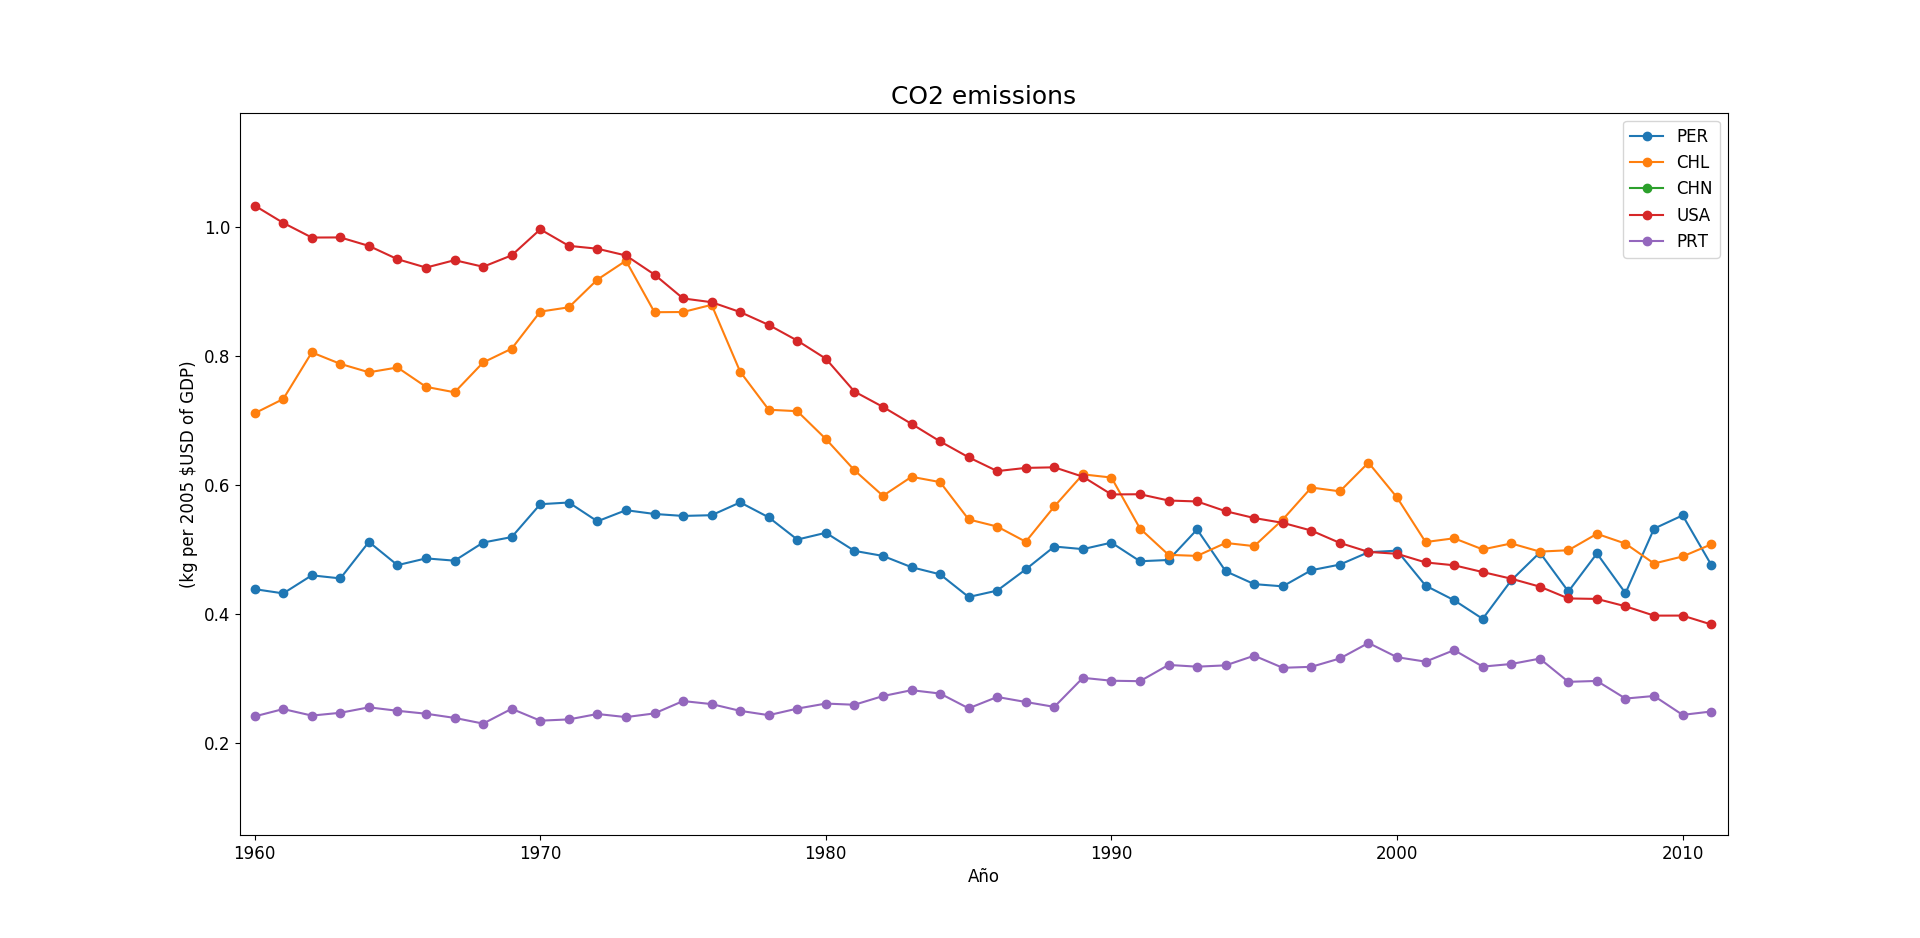
\includegraphics[scale=0.38]{images/zoom - co2.png}
	\caption{Emisiones de CO2: Zoom.}
	\label{fig:11}
\end{figure}

\begin{figure}
	\centering
	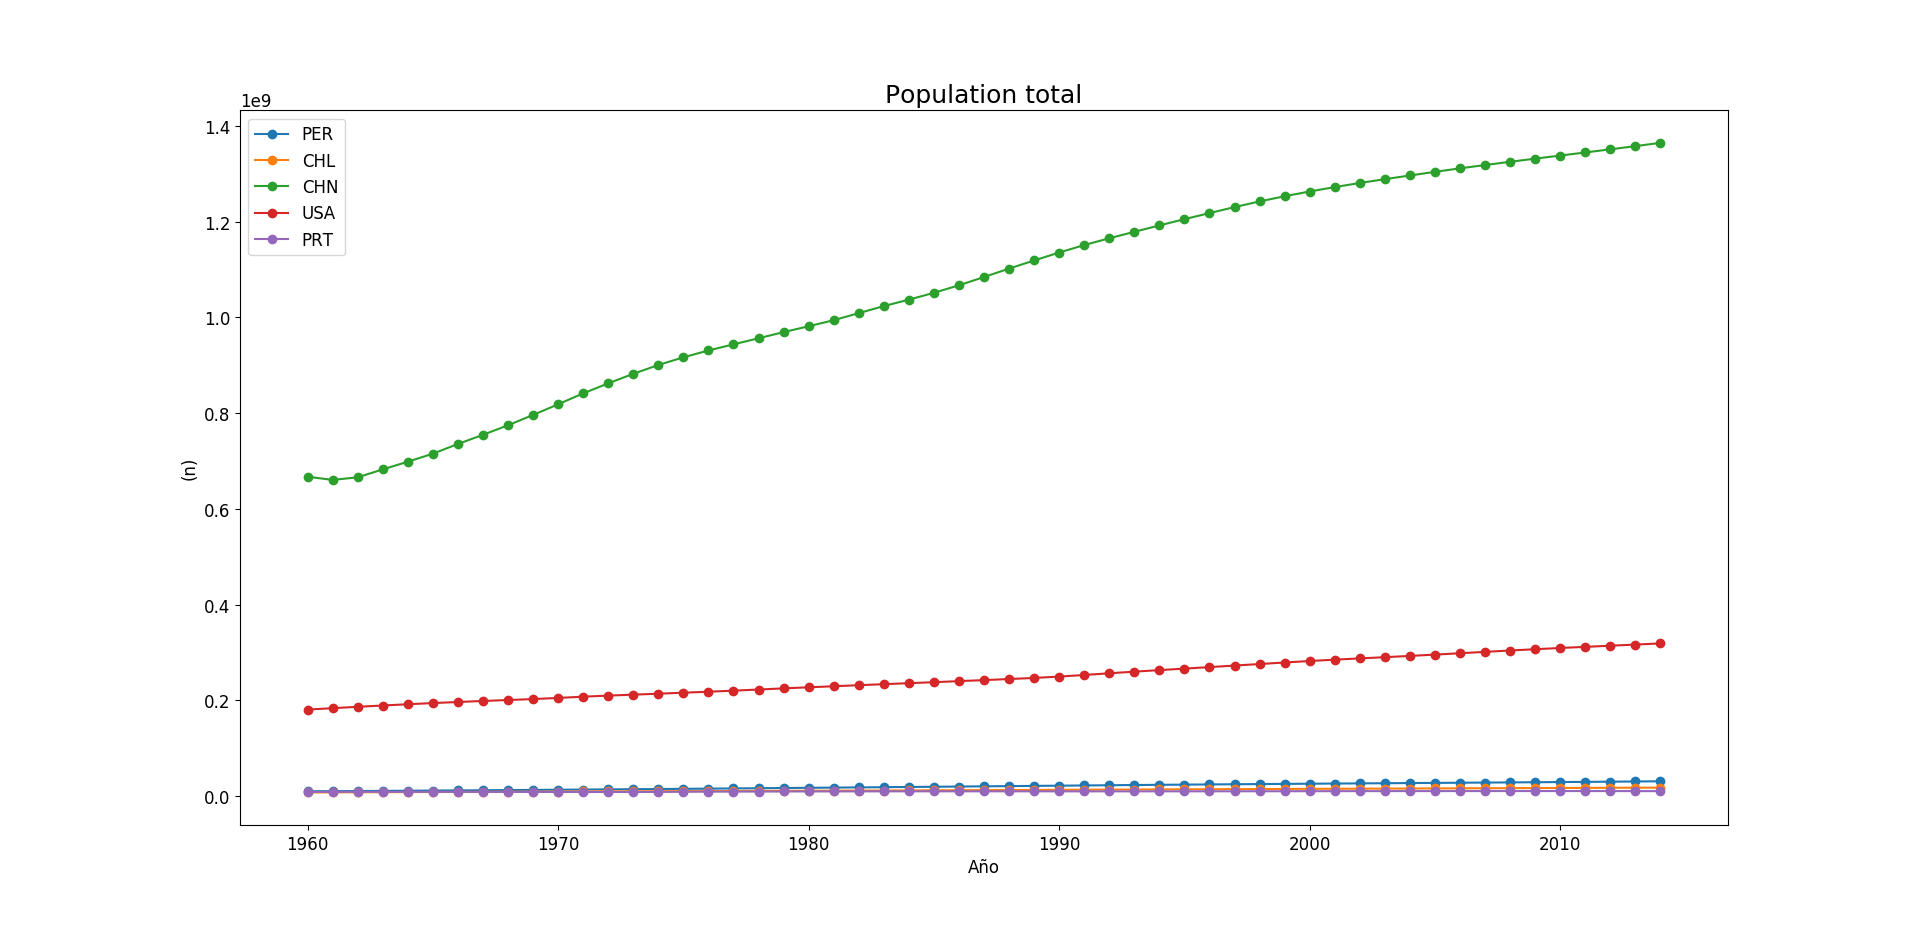
\includegraphics[scale=0.38]{images/populationtotal.png}
	\caption{Población total.}
	\label{fig:12}
\end{figure}

\begin{figure}
	\centering
	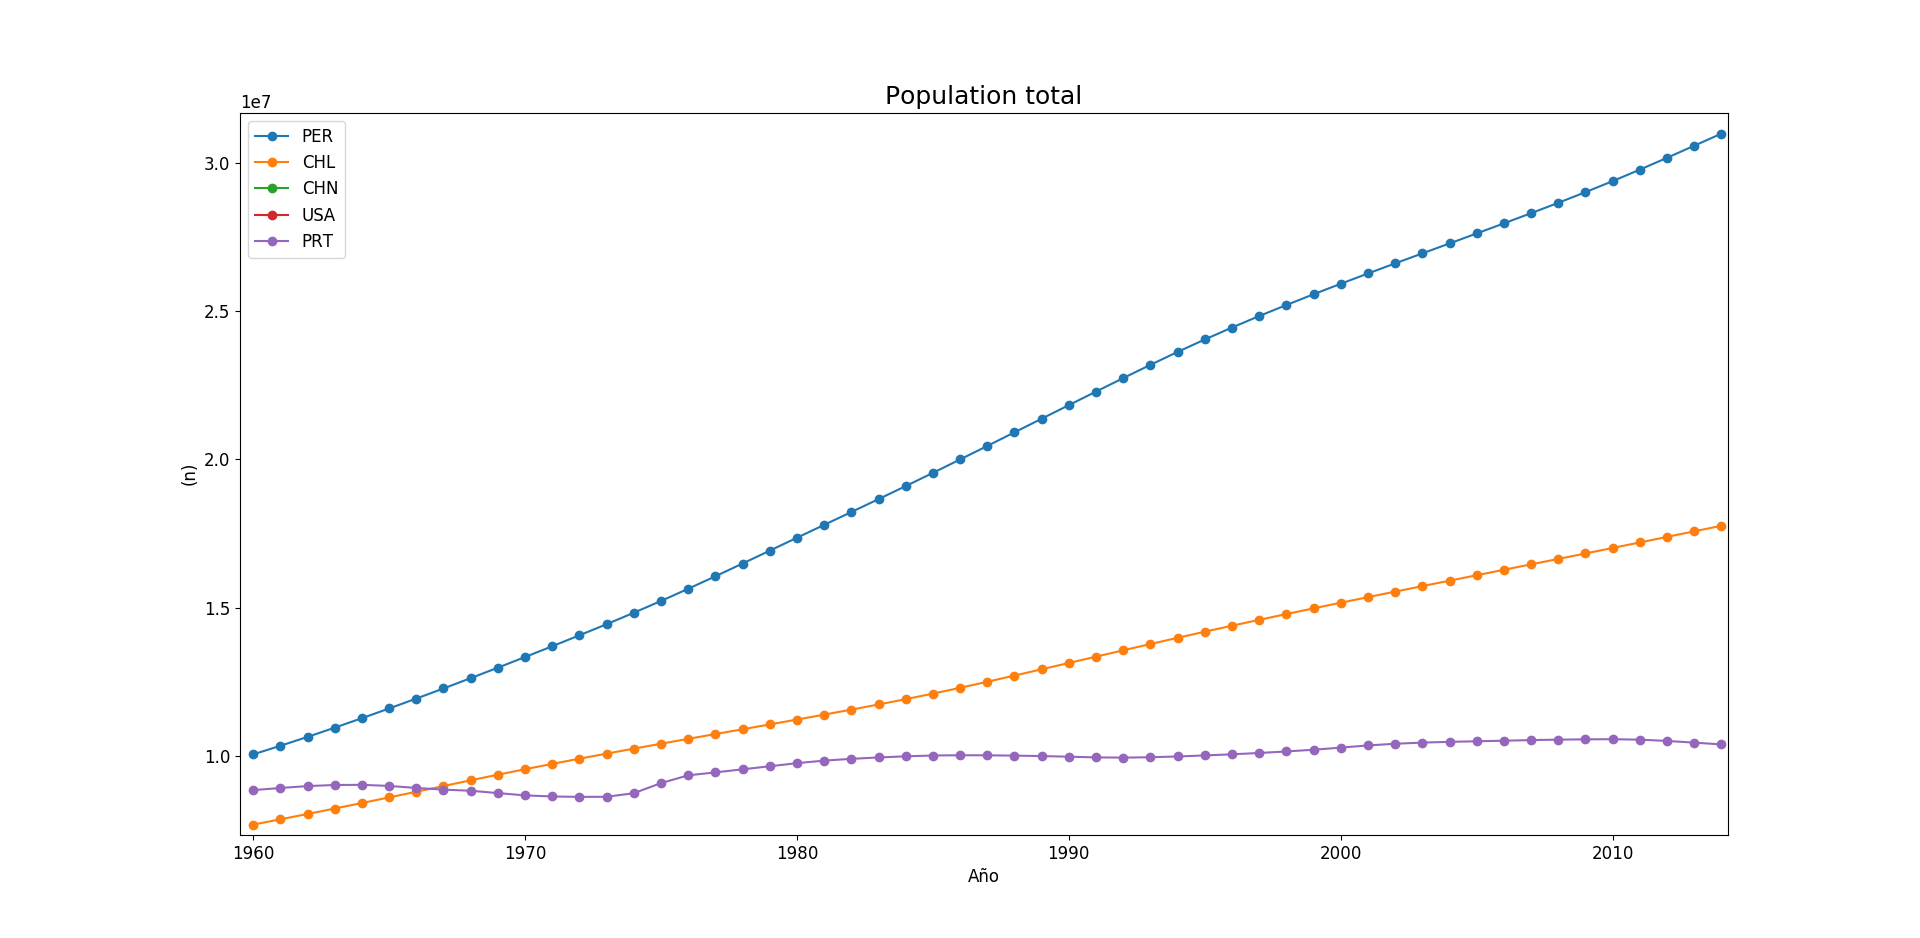
\includegraphics[scale=0.38]{images/pt-zoom.png}
	\caption{Población total: Zoom.}
	\label{fig:13}
\end{figure}





\end{document}